% Artyom Voronin
%           _                     
% _ __ ___ | |__  _ __  _ __ ___  
%| '_ ` _ \| '_ \| '_ \| '_ ` _ \ 
%| | | | | | |_) | |_) | | | | | |
%|_| |_| |_|_.__/| .__/|_| |_| |_|
%                |_|              
%
% Brno, 2021


\chapter{PdM using a Simulation Model}\label{ch:mb}
This chapter deals with model-based methods and the possibilities of using
a simulation model to design and develop a PdM algorithm.  Section
\ref{sec:diffs_mb_dt} presents the difference between model-based PdM and
PdM using the simulation model as a digital twin.  A demonstration of the
possibility of generating sensor fault conditions is demonstrated in
section \ref{sec:sensor_fault_generation}.  Using identified
Hammerstein-Weiner model to extract condition indicators in the form of a
dynamic system parameter shown in section \ref{sec:mb_hw_demo}.  In section
\ref{sec:residuals}, the simulation model is used as a nominal, and
residual estimation is performed with the following training of the
classification model.  The left sections \ref{sec:mb_rul} deal with the use
of a simulation model to generate degradation data. And the use of a newly
generated dataset to estimate the remaining useful life.


\section{Differences between Model-Based PdM and PdM using Digital Twin}\label{sec:diffs_mb_dt}
There is a difference between using Model-Based PdM and using Simulation
Model as a Digital Twin.

\section{Using Digital Twin to Generate Fault Data}\label{sec:sensor_fault_generation}
We can use Digital Twin to model situations that were not captured in the
original dataset or if it is hard to model some cases with real-world
hardware. As an example, we can model sensors fault such as sensor drift or
complete signal loss.

\subsection{Sensor Fault Modeling}

\begin{figure}[h!]
    \centering
    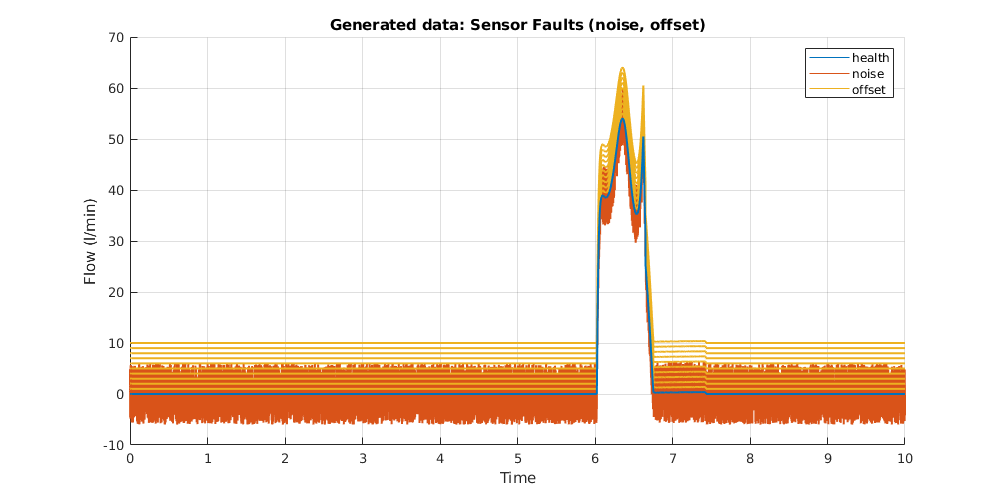
\includegraphics[width=1\textwidth]{mb_sensor_signal.png}
    \caption{Caption}
    \label{fig:}
\end{figure}

\begin{figure}
    \centering
    \begin{subfigure}[b]{0.45\textwidth}
        \centering
        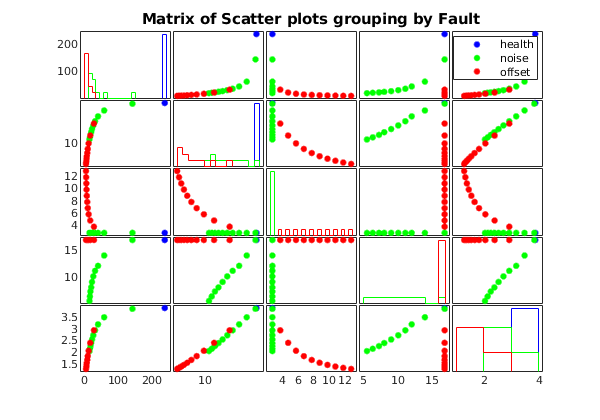
\includegraphics[width=1.2\textwidth]{mb_sensor_matrix.png}
        \caption{Caption}
        \label{fig:}
    \end{subfigure}
    \hfill
    \begin{subfigure}[b]{0.45\textwidth}
        \centering
        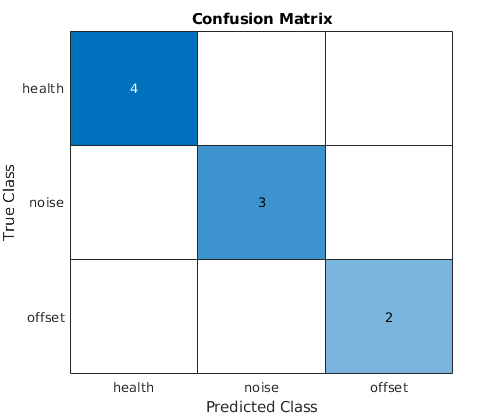
\includegraphics[width=1\textwidth]{mb_sensor_conf.png}
        \caption{Caption}
        \label{fig:}
    \end{subfigure}
    \caption{Caption}
    \label{fig:}
\end{figure}



\section{Model-Based Condition Indicators}
Model-Based approach is suitable when it's difficult to identify condition
indicators using only signals. In some cases it's useful to fit some model
from data and extract condition indicators as some system parameter.

\subsection{Static and Dynamic Models}
If the system behavior can be fit from the data as a static model, than we
can extract condition variables from this model. For example, if model
was fitting to a polynomial model, than polynomial coefficients can be use
as condition indicators.

Signals showing dynamic behavior can be fitted to dynamic models such as
State-Space or AR, ARX, NLARX (Nonlinear auto recursive model) and so on.
Then condition indicators can be extracted as poles, zeros damping
coefficients from estimated model.

\subsection{Using Hammerstein-Wiener Model}\label{sec:mb_hw_demo}
Demo using Hammerstein-Wiener Model. Fit model to position signal and
extract coefficients from model as Condition indicators. Classification.

\begin{figure}[h!]
    \centering
    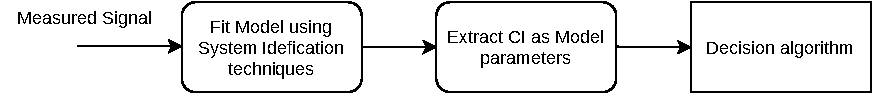
\includegraphics[width=0.8\textwidth]{mb_hw.pdf}
    \caption{Caption}
    \label{fig:}
\end{figure}


\section{Using Simulation Model for Residuals Estimation}\label{sec:residuals}

Another option is using the Simulink model with \textbf{prediction
error minimization function} to compute difference between Simulink model
and measured data. From this difference we can separate fault condition and
healthy operation. 

\begin{figure}[h!]
    \centering
    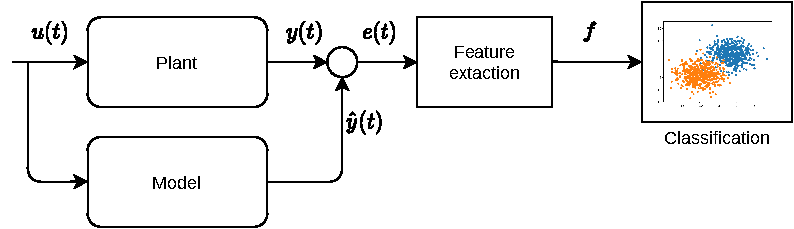
\includegraphics[width=0.7\textwidth]{mb_resid.pdf}
    \caption{Caption}
    \label{fig:}
\end{figure}


Compare actual system behavior with system model. This will generate some
error $e(t) = y(t) - \hat{y}(t)$. From this error residual can be generated
in form $r(t)=\Phi(u_t,y_t, \varepsilon_t,v_t,d)$ and after some decision.

\begin{figure}[h!]
    \centering
    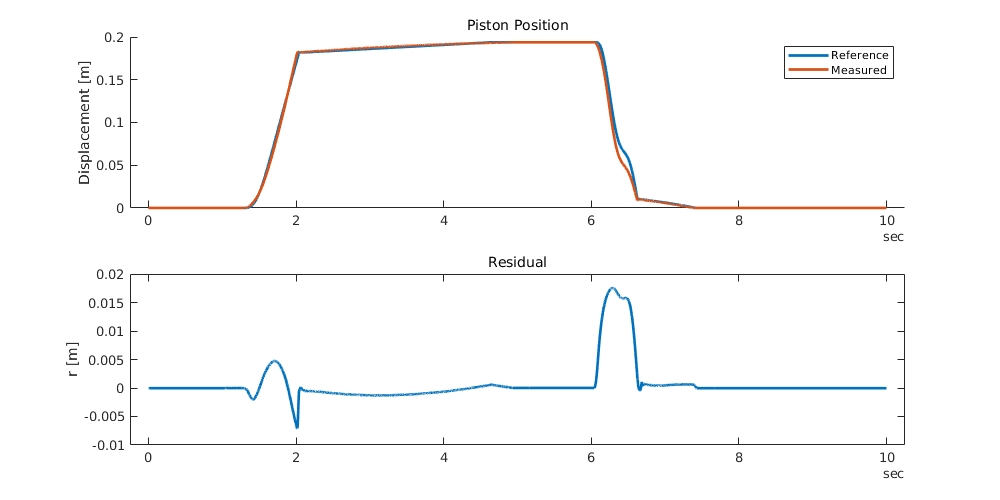
\includegraphics[width=1\textwidth]{mb_resid_signal.png}
    \caption{Caption}
    \label{fig:}
\end{figure}



\begin{table}[h!]
    \centering
    \begin{tabular}{|c|c|c|}
        \hline
          &        Features               & Kruskal-Wallis \\ \hline
        1 &   LeverPosition\_res\_stats/RMS	    & 543.82 \\ \hline  
        2 &   LeverPosition\_res\_stats/PeakValue	& 271.94 \\ \hline  
        3 &   LeverPosition\_res\_stats/Std	    & 222.89 \\ \hline  
        4 &   LeverPosition\_res\_stats/THD	    & 215.34 \\ \hline  
        5 &   LeverPosition\_res\_stats/Kurtosis	& 129.66 \\ \hline  
        \hline
    \end{tabular}
    \caption{First Five Ranked Condition Indicators using ANOVA}
    \label{tab:resid_sorted_ci}
\end{table}

\begin{figure}[h!]
    \centering
    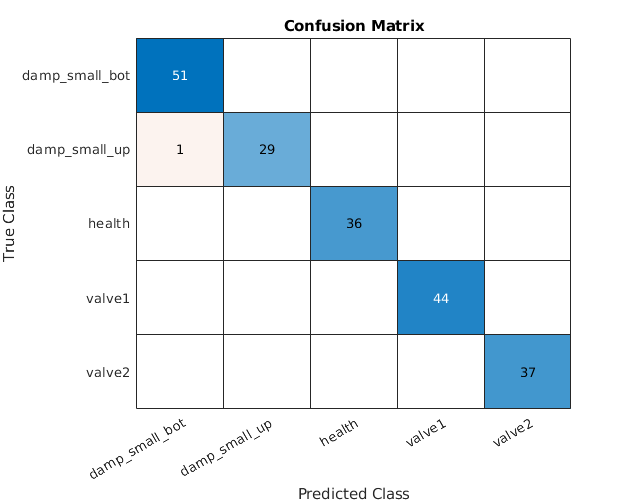
\includegraphics[width=0.5\textwidth]{mb_resid_conf.png}
    \caption{Caption}
    \label{fig:}
\end{figure}





\section{Using Digital Twin to Generate Prognostic Data}\label{sec:mb_rul}
Another option is to use Digital Twin to generate a system degradation
process. We can evaluate CI from sensor signal by changing a system's
mechanical properties as friction or mass flow leakage.  Another advantage
is that we can design experiments on the model to evaluate what type of
data we require from a real-world system to develop a robust algorithm.


\subsection{Air Leak Modeling}
\todo[inline]{Air leak model add math + pressure plot}


\section{RUL}
\subsection{Prognostic CI}
\begin{figure}[h!]
    \centering
    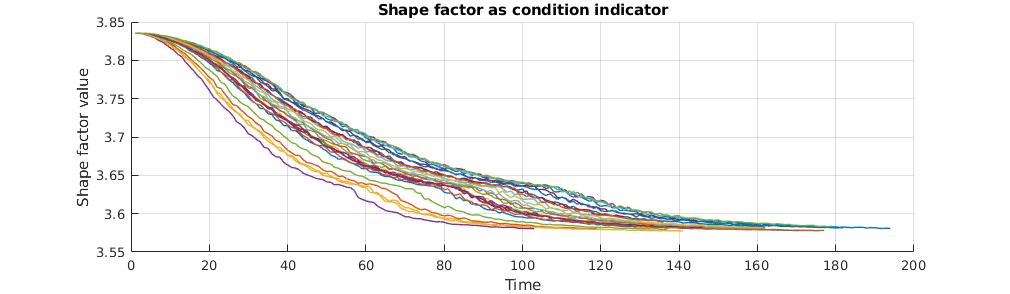
\includegraphics[width=1\textwidth]{rul_ci.png}
    \caption{Caption}
    \label{fig:}
\end{figure}


\subsection{RUL Models}

\begin{figure}
    \centering
    \begin{subfigure}[b]{0.55\textwidth}
        \centering
        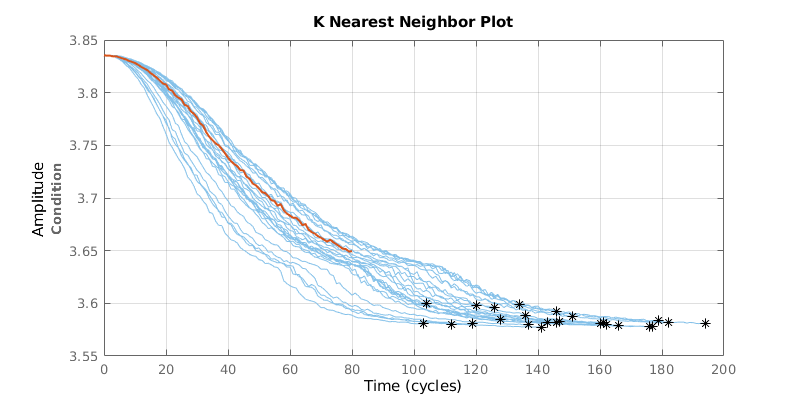
\includegraphics[width=1.2\textwidth]{rul_resid_model_knn.png}
        \caption{Caption}
        \label{fig:}
    \end{subfigure}
    \hfill
    \begin{subfigure}[b]{0.4\textwidth}
        \centering
        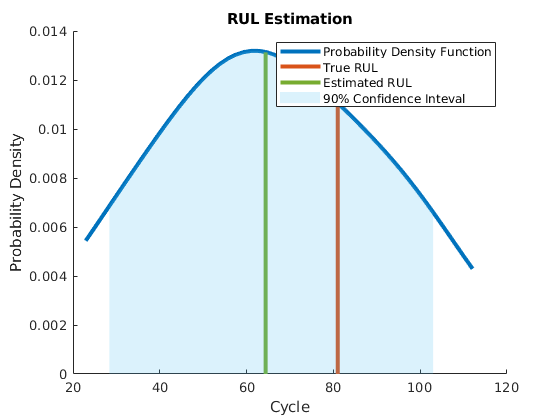
\includegraphics[width=1.1\textwidth]{rul_resid_model_pdf.png}
        \caption{Caption}
        \label{fig:}
    \end{subfigure}
    \caption{Caption}
    \label{fig:}
\end{figure}


Demo RUL using generated from model degradation dataset.

RUL linear degradation model:
\begin{figure}[h!]
    \centering
    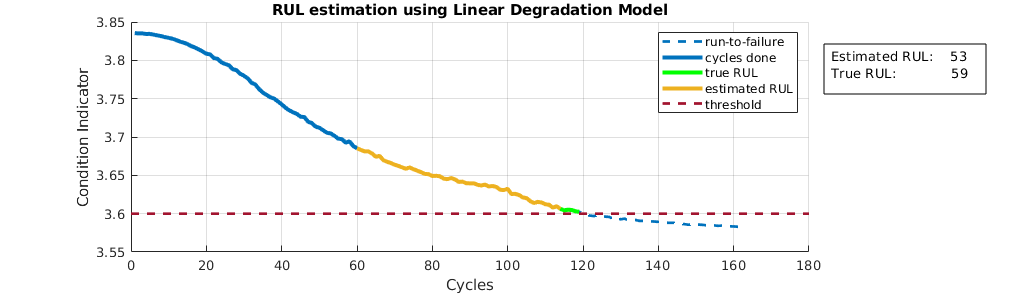
\includegraphics[width=1\textwidth]{rul_final.png}
    \caption{Caption}
    \label{fig:}
\end{figure}


\todo[inline]{Text}
\lipsum
